\section{Moduł ATRIAL\_FIBR}
\subsection{Badania literaturowe}
Celem jest wykrycie u osoby badanej migotania przedsionków (ang. \textit{Atrial Fibrillation}). 
Jest to zaburzenie polegające na nieskoordynowanym pobudzeniu przedsionków serca. 
Ryzyko zgonu u osoby chorej wzrasta dwukrotnie, a problem dotyczy $1-2\%$ ogółu populacji.
Migotanie przedsionków zazwyczaj jest bezobjawowe, zaburzenie jest wykrywane przypadkowo,
lub po udarze niedokrwiennym mózgu.
Zwykle występuje u pacjentów z organiczną chorobą serca, ale również może wystąpić u osób zdrowych.
Możliwe do zaobserwowania objawy to duszności, kołatanie serca, ból w klatce piersiowej czy zawroty głowy.

Sygnał EKG u chorego charaktreryzuje się następującymi własnościami:
\begin{itemize}
  \item brak załamków P
  \item odstępy R-R nieregularne
  \item obecna fala migotania
  \item zespoły QRS zwykle wąskie
\end{itemize}
\begin{figure}[ht]
\centering
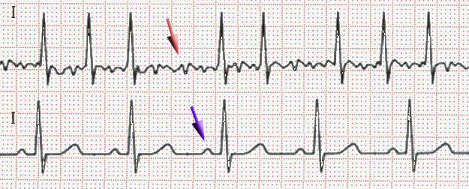
\includegraphics{ATRIAL_FIBR/img/AF_ecg.jpg}
\label{fig:AF_ecg}
\caption{Sygnał EKG dla osoby chorej i prawidłowy rytm zatokowy}
\end{figure}

Rysunek~\ref{fig:AF_ecg} na górym zapisie przedstawia sygnał EKG dla osoby chorej na migotanie przedsionków,
natomiast dolny zapis prezentuje prawidłowy rytm zatokowy.
Wykres osoby chorej wyraźnie przedstawia wszystkie podane symptomy.

Literatura podawała kilka czynników mogących wskazywać na występowanie u pacjenta migotania przedsionków. 
Jeden artykuł [1] przedstawiał metodę opartą jedynie na detekcji peaków R. 
Autorzy uważali, że na podstawie jedynie nieregularnych interwałów R-R 
można z powodzeniem wykryć u badanego chorobę. 
Metoda ta polega na zaklasyfikowanie odległości jako małych, dużych i normalnych. 
Następnie przedstawienie jako procesu Markowa i porównanie do wyników osoby zdrowej miało pozwolić 
na uzyskanie ostatecznego wyniku.
Niestety, po wyliczeniu parametrów dot. bicia serca, 
okazało się, że jeden z próbnych sygnałów dostępnych w bazie Physiobank - 
iaf4\_ivc - wykazuje własności bardzo zbliżone do zdrowego człowieka.

Autorzy drugiego źródła [2], prócz wspomnianej rozszerzyli sposób rozwiązania problemu dodając następujące metody:
\begin{enumerate}
 \item \textbf{Wykrycie absencji załamka P}
 
    Po ustaleniu pewnego wzorca  P (na podstawie dużej liczby próbek), 
    zostaje porównany do sygnału osoby badanej. 
    Ilość wystąpień załamka zostaje wyznaczona na podstawie wyznaczonego progu.
 \item \textbf{Analiza aktywności przedsionków}
 
    Po usunięciu QRS-T, sygnał u osoby chorej charakteryzuje się występowaniem fali o częstotliwości 4-10 Hz. 
    Należy wykonać analizę widma -- po zastosowaniu FFT (Fast Fourier Transform) 
    trzeba sparametryzować widmo częstotliwości.  
    U osoby chorej można zaobserwować koncentrację wokół wierzchołka położonego w przedziale [4,10] Hz.
\end{enumerate}

\subsection{Koncepcja proponowanego rozwiązania}
Początkowo zasugerowani artykułem z MIT postanowiliśmy wypróbować metodę tam przedstawioną 
i ograniczyć się do analizy interwałów R-R. 
Jednak po niepowodzeniu zmuszeni byliśmy wybrać inną metodę. 
Ze względu na istotę problemu -- zdecydowaliśmy się również wykorzystać metodę wykrywania absencji P.
\paragraph{Analiza sygnału będzie więc polegała na zbadaniu występowania 2 parametrów:}
\begin{enumerate}
    \item Odległości pomiędzy załamkami R
    \item Brak załamków P
\end{enumerate}
Gdy oba warunki zostaną spełnione, uznamy, że występuje migotanie przedsionków w danym sygnale.

\paragraph{Parametry związane z rytmem serca}
Informację na temat położenia w czasie peaków R otrzymamy z modułu QRS Complex. 
Na jej podstawie zakwalifikujemy każdy przedział RR jako krótki (poniżej 85\% średniej), 
średni, oraz długi (powyżej 115\% średniej). 
Następnie wyliczymy prawdopodobieństwo przejść między poszczególnymi stanami. 
Finalnie otrzymamy z tego dwa parametry - 
entropię sygnału oraz odchylenie sygnału od średniej macierzy zdrowego człowieka metodą Jensena-Shannona.
\begin{figure}[ht]
\centering
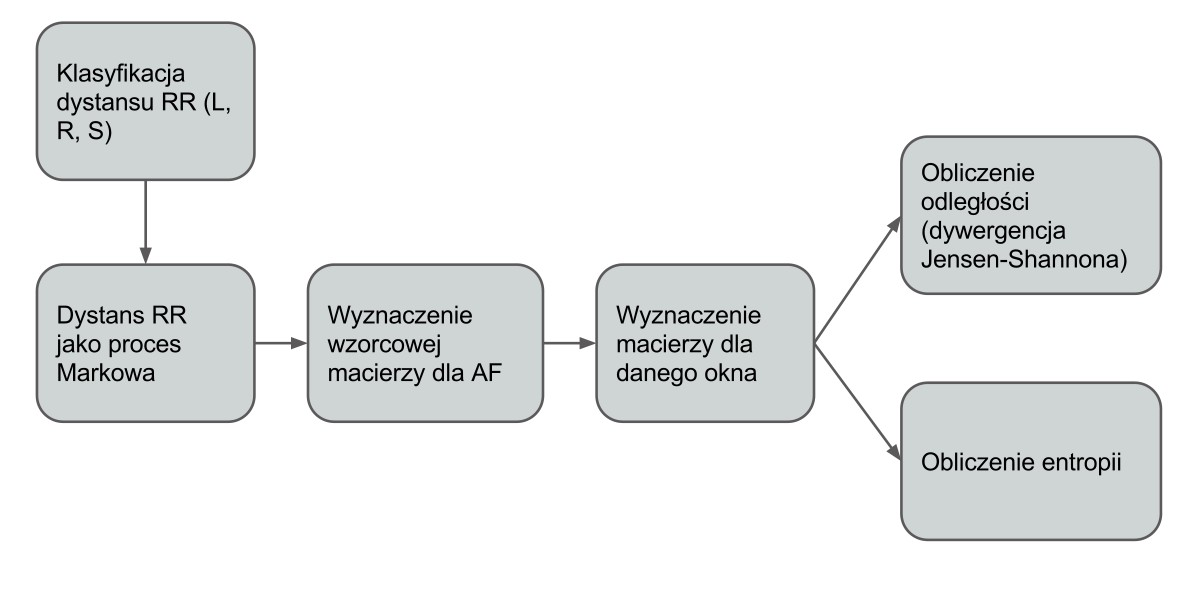
\includegraphics[width=12cm]{ATRIAL_FIBR/img/RRMethodFlow.jpg}
\end{figure}

\begin{table}[!ht]
  \centering
  \begin{tabular}{|r|ccc|}
    \hline 
    & S & M & L \\
    \hline
    S & 0.005 & 0.023 & 0.006 \\
    M & 0.007 & 0.914 & 0.013 \\
    L & 0.019 & 0.006 & 0.003 \\
    \hline
  \end{tabular}
  \caption[Macierz Markowa - zdrowy człowiek]
          {Prawdopodobieństwo zmiany długości dystansu RR w przypadku zdrowego człowieka. 
            S - dystans krótki (mniej niż 85\% średniego), 
            M - średni, L - długi (ponad 115\% średniego)}
\end{table}

\begin{table}[!ht]
  \centering
  \begin{tabular}{|r|ccc|}
    \hline 
    & S & M & L \\
    \hline
    S & 0.056 & 0.114 & 0.062 \\
    M & 0.101 & 0.350 & 0.096 \\
    L & 0.060 & 0.114 & 0.035 \\
    \hline
  \end{tabular}
  \caption[Macierz Markowa - chory człowiek]{Uśredniona macierz Markowa dla ludzi chorych na migotanie przedsionków}
\end{table}

Prawdopodobieństwo przejścia ze stanu R (regular) do kolejnego R wynosi:
\begin{equation}
P(R|R) = \frac{P(R,R)}{P(R)}
\end{equation}

Jako miary opisującej odległość między macierzami początkowo, zgodnie z zaleceniami pozycji \cite{Pedrycz}, 
chcieliśmy użyć dywergencji Kullbacka-Leiblera:
\begin{equation}
F_{KL}(P(E_i,E_j),\overline{P_{AF}(E_i,E_j)}) = \sum_{i=1}^3\sum_{j=1}^3P(E_j, E_j) \log\left(\frac{P(E_i, E_j)}{P_{AF}(E_i,E_j)} \right)
\end{equation}
natomiast ze względu na to, że jest asymetryczna, czyli de facto nie jest metryką, postanowiliśmy skorzystać z dywergencji \textbf{Jensena-Shannona}. 
Bazuje na powyższej dywergencji, z pewnymi znaczącymi różnicami.
Jest symetryczna i zawsze ma skończoną wartość.
Pierwiastek kwadratowy dywergencji Jensena-Shannona jest metryką zwaną dystansem Jensena-Shannona.
\begin{equation}
F_{JS} = \frac{1}{2}F_{KL}(P(E_i,E_j),M)+\frac{1}{2}F_{KL}(\overline{P_{AF}(E_i,E_j)},M)
\end{equation}
gdzie $$M = \frac{1}{2}(P(E_i,E_j)+\overline{P_{AF}(E_i,E_j)})$$

W przypadku entropii skorzystaliśmy ze standardowej definicji:
\begin{equation}
H = \sum_{i=1}^3 P(E_j|E_i) 
\end{equation}

\begin{equation}
H(E_j) = - \sum{j=1}^3P(E_j|E_i)\log_2P(E_j|E_i)
\end{equation}
Metoda została przez nas wstępnie przetestowana przy użyciu aplikacji napisanej w języku programowania Julia. 
Pozwoliło to nam wysnuć pierwsze wnioski z wykresu~\ref{fig:RRResults}.
Zielone kropki przedstawiają parametry dla sygnałów z bazy Physiobank zebranych od zdrowych ludzi,
czerwone natomiast pochodzą od chorych na migotanie przedsionków. 
Niestety nie jest możliwe oddzielenie puli kropek zielonych od czerwonych jedną linią, 
dlatego potrzebujemy dodatkowego parametru.

\begin{figure}[ht]
\centering
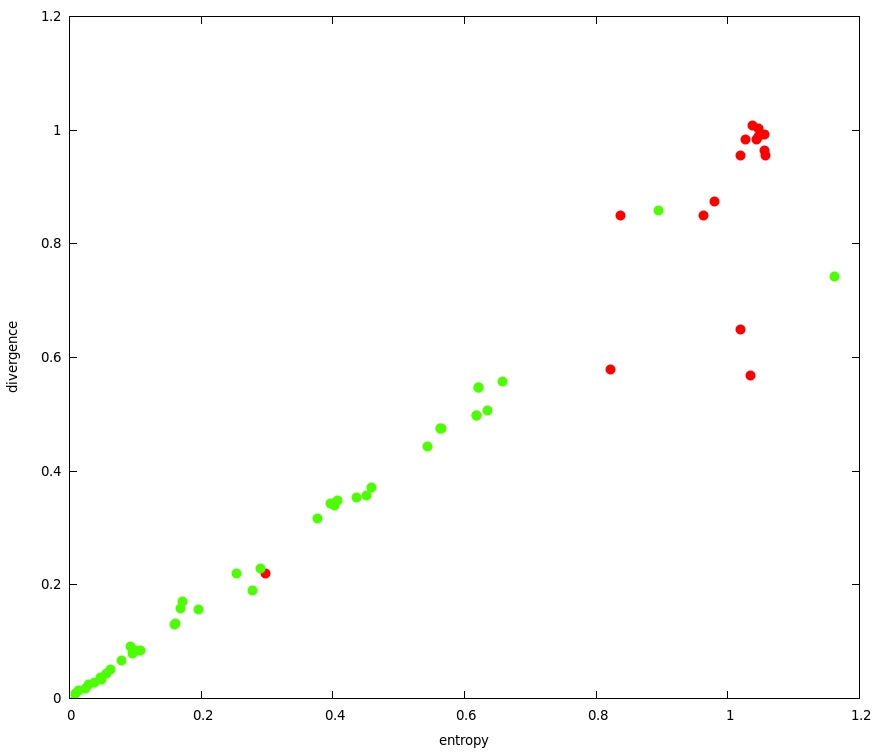
\includegraphics[width=12cm]{ATRIAL_FIBR/img/RRResults.jpg}
\caption{Entropia i dywergencja dla danych Physiobank}
\label{fig:RRResults}
\end{figure}

\paragraph{Detekcja absencji P}
Z modułu WAVES otrzymamy informację na temat położenia początkowego i końcowego załamka P. 
Na tej podstawie wyliczymy średni przebieg tej fali u zdrowego człowieka. 
Następnie przy użyciu oszacowanego progu wyliczymy procentową absencję fali P w zadanym sygnale, 
która będzie stanowiła kolejny współczynnik.
\begin{figure}
  \centering
  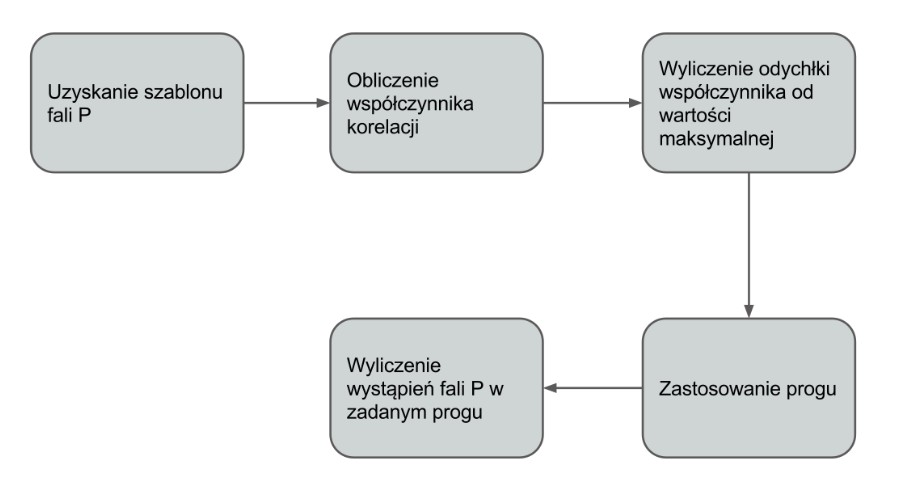
\includegraphics[width=12cm]{ATRIAL_FIBR/img/PWaveFlow.jpg}
  \caption{Algorytm wyliczenia współczynnika występowania fali P.}
\end{figure}

Wyliczenie współczynnika korelacji:
\begin{equation}
cc(i) = |\mathrm{corr\:coef}(P_\mathrm{wave}(i),\: \overline{P_\mathrm{wave}(i)})|, \quad i = 1,\ldots,n\; \mathrm{beats}
\end{equation}
\begin{equation}
  |\mathrm{corr\:coef}(x,y)| = 
  \frac
      {\sum_{i=1}^{n}(x(i) - \overline{x})(y(i) - \overline{y})}
      {
        \sqrt{\sum_{i=1}^{n}(x(i) - \overline{x})}
        \sqrt{\sum_{i=1}^{n}(y(i) - \overline{y})}
      }
\end{equation}
Za wykrytą falę P uznajemy tę, dla której współczynnik korelacji wynosi co najmniej $0.2$.
Stosunek liczby wykrytych fal P do liczby wszystkich okresów PQRST jest poszukiwanym współczynnikiem.

\subsection{Rezultaty i wnioski}
Zaproponowane przez nas metody zostały poprawnie zaimplementowane w języku C++ oraz zintegrowane z główną linią projektu.
Integralną częścią dostarczonego przez zespół kodu był zestaw testów jednostkowych napisanych 
z wykorzystaniem frameworka QtTest.

Zgodnie z koncepcją proponowanego rozwiązania, ocena prawdopodobieństwa zachorowania pacjenta na migotanie przedsionków
jest średnią ważoną z następujących parametrów:
\begin{itemize}
 \item \textbf{Dywergencja Jensena-Shannona} między wzorcową macierzą Markowa opisującą prawdopodobieństwo przejść między stanami,
 a macierzą wyliczoną dla danego pacjenta. 
 Dywergencja $0$ oznacza, że macierz jest identyczna z wzorcową. 
 
 \item \textbf{Entropia macierzy Markowa}.
 Wartość $0$ oznacza, że wszystkie wartości dystansów między falami R mieszczą się w przedziale $[85\%,115\%]$ wartości średniej.
 Z drugiej strony, wartość $1$ mówi o dużej nieregularności występowania fali R, 
 co jest symptomatyczne dla osób cierpiących na migotanie przedsionków.
 
 \item \textbf{Współczynnik zaniku fali P}. 
 Stosunek liczby okresów PQRST w których fala P występuje, do całkowitej liczby tych okresów.
 Za występowanie fali P uznajemy sytuację, w której korelacja między sygnałem w przedziale otrzymanym z modułu WAVES,
 a sygnałem wzorcowym jest większa od $0.2$.
\end{itemize}
Po zaaplikowaniu wyżej wspomnianych metod dla wzorcowych sygnałów z bazy Physiobank, 
można stwierdzić, że program dokonuje detekcji poprawnie. 
Właściwie dla wiekszości przypadków wystarczająca jest sama analiza rytmu bicia serca (dystansów R-R).
Zastosowanie drugiej metody związanej z absencją fali P dodatkowo zwiększyło skuteczność wykrywania choroby.

